\chapter{Refining Heuristics}
In this chapter are discussed the heuristic that starting from an initial solution of the TSP, return a better solution in term of cost. This kind of heuristic will be called Refining Heuristics because of the solution cost improvement. 

\section{2-opt} \label{sec:best_2_opt}

This heuristic is a simple and effective local search algorithm for TSP problem.\\
A pseudo-code is proposed in alg. \ref{alg:2opt} to describe how it works. The input parameter $ T $ is an ordered list of edges that define a tour and each edge is represented with an ordered pair of nodes. The \texttt{swap\_edges} method remove the two input edges from the tour $ T $ and add the new edges as show in fig. \ref{fig:2_opt_graph}.

\begin{algorithm}
	\caption{}\label{alg:2opt}
	\begin{algorithmic}[1]
	\Procedure{Procedure 2\_opt}{T}
		\State{\textit{// Variable initialization}}
		\State{$ (n_1, n_2), (m_1, m_2) = T[1], T[3] $}
		\State{$ (n_1^*, n_2^*), (m_1^*, m_2^*) = (n_1, n_2), (m_1, m_2) $}
		\State{$ \delta_{cost}^* = c_{n_1m_1} + c_{n_2m_2} - c_{n_1n_2} - c_{m_1m_2}  $}
		\For{$ (n_1,n_2) \in T $}
			\For{$ (m_1,m_2) \in T $ } \textit{ // For each pair of edge in the tour}
				\If{$ n_1 == m_1 \lor n_1 == m_2 \lor n_2 == m_1 \lor n_2 == m_2 $}
					\State{\textbf{continue}}
				\EndIf
				\State{$ \delta_{cost} = c_{n_1m_1} + c_{n_2m_2} - c_{n_1n_2} - c_{m_1m_2} $}
				\If{$ \delta_{cost} < \delta_{cost}^* $} \textit{ // Find 2-opt candidates}
					\State{$ \delta_{cost}^* = \delta_{cost} $}
					\State{$ (n_1^*, n_2^*), (m_1^*, m_2^*) = (n_1, n_2), (m_1, m_2) $}
				\EndIf
			\EndFor
		\EndFor
		\State{\texttt{swap\_edges($ T, (n_1^*, n_2^*), (m_1^*, m_2^*) $)}}
	\EndProcedure
	\end{algorithmic}
\end{algorithm}

In the example in fig. \ref{fig:2_opt_graph} the pair that has the best improvement is $ (1,4) $ and $ (5,2) $. Note that although $ (5,2) = (2,5) $ for the model, to be coherent with $ \delta_{cost} $ annotation, an orientation of the tour must be choose, and each edge must be represented with consequent ordered node pair: if $ (1,4) $ is the first considered edge, it impose the orientation of the tour.

\begin{figure}[h]
	\centering
	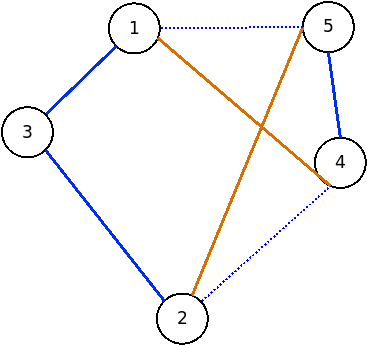
\includegraphics[width=.3\columnwidth]{img/2_opt_graph.png}
	\caption{Example graph to explain \texttt{2\_opt} method. The input graph is that with continuous edges. \texttt{2\_opt} would remove $ (1,4) $ and $ (2,5) $ from the tour and replace them with $ (1,5) $ and $  (2,4) $}
	\label{fig:2_opt_graph}
\end{figure}
As can be seen in fig. \ref{fig:lb_time_grasp_best_two_opt_d2103} multiple execution of \texttt{2\_opt} can improve more than 50\% the cost of the solution before to find a local minimum. This method in the report is called \texttt{best\_two\_opt}.
\begin{figure}[!h]
\centering
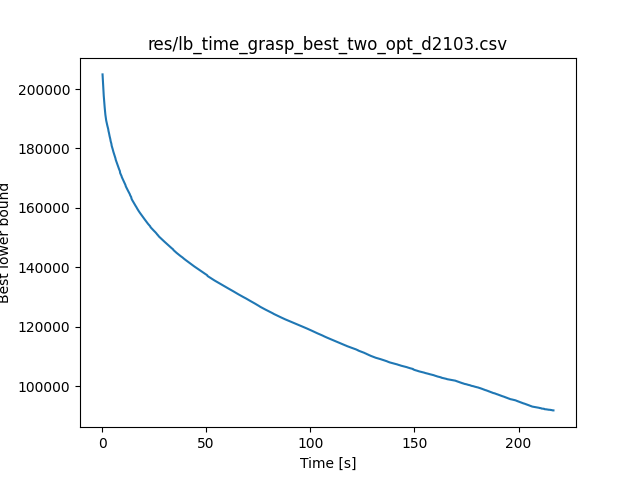
\includegraphics[width=.6\columnwidth]{../res/lb_time_grasp_best_two_opt_d2103.png}
\caption{Solution cost profile of \texttt{best\_two\_opt}. \texttt{GRASP} solution is used as warm start.}
\label{fig:lb_time_grasp_best_two_opt_d2103}
\end{figure}

It is interesting to see the solution cost profile of \texttt{best\_two\_opt} (fig. \ref{fig:a280_25}) applied to the best of the Greedy solutions (called \texttt{greedy\_best\_two\_opt}). The improve of the cost solution is considerable even if it stop on a local minimum.  Note that, the best tour is calculated in about $ 8 $s with \texttt{subtour\_callback\_general}, \texttt{Greedy} take about $ 5 $s to find the \texttt{Greedy} tours and \texttt{best\_two\_opt} find a local minimum in $0.07$s. Moreover is important to consider that \texttt{Greedy} method can be easily modify to execute each Greedy tour in parallel and than apply \texttt{best\_two\_opt}.\\
In fig.s \ref{fig:a280_10} and \ref{fig:a280_25} can be compared the \texttt{Greedy}, \texttt{greedy\_best\_two\_opt} and \texttt{subtour\_callback\_general} tours, solutions cost and execution time.\\

\begin{figure}[!h]
	\begin{subfigure}{.5\columnwidth}
		\centering
		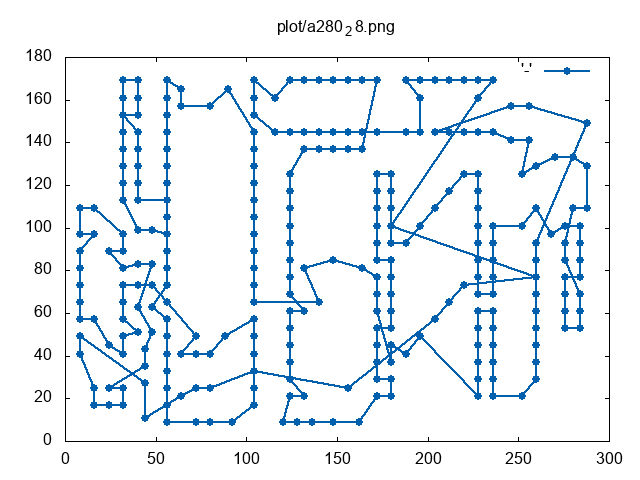
\includegraphics[width=\columnwidth]{../res/a280_28.png}
		\caption{\texttt{n\_greedy\_10}: cost=3078, time=0.45s}
		\label{fig:a280_10}
	\end{subfigure}
	\begin{subfigure}{.5\columnwidth}
		\centering
		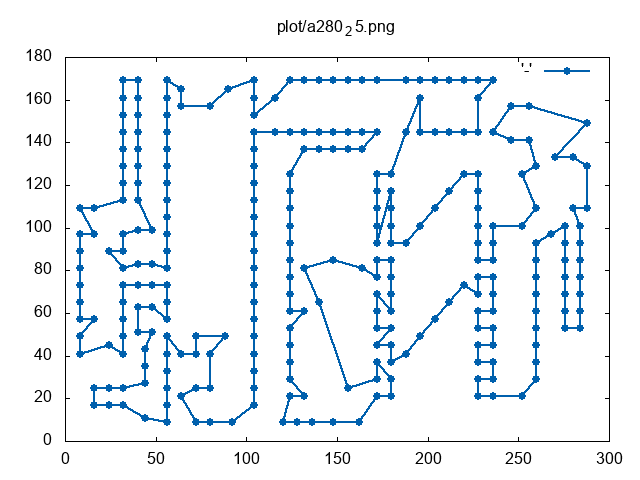
\includegraphics[width=\columnwidth]{../res/a280_25.png}
		\caption{\texttt{n\_greedy\_best\_two\_opt}: cost=2683, time=0.06s}
		\label{fig:a280_25}
	\end{subfigure}
	\begin{subfigure}{.5\columnwidth}
		\centering
		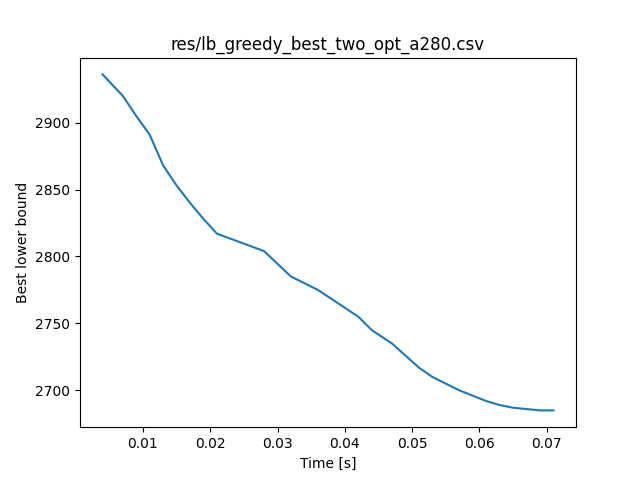
\includegraphics[width=\columnwidth]{../res/lb_greedy_best_two_opt_a280.png}
		\caption{The profile of the solution cost over time of the \texttt{best\_two\_opt} optimization phase.}
		\label{fig:lb_greedy_best_two_opt_a280}
	\end{subfigure}
	\begin{subfigure}{.5\columnwidth}
		\centering
		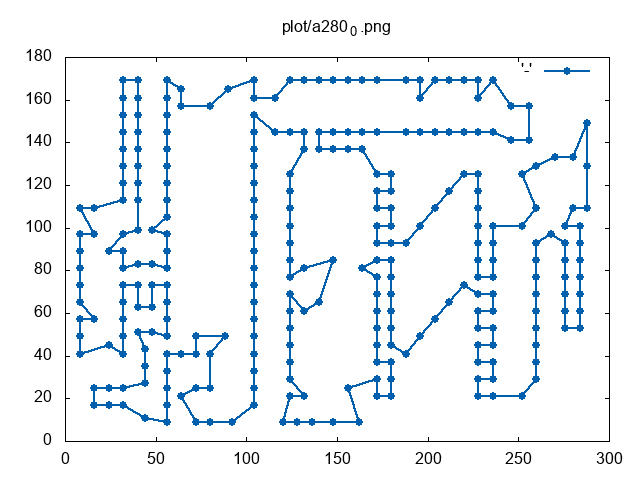
\includegraphics[width=\columnwidth]{../res/a280_0.png}
		\caption{\texttt{subtour\_callback\_general}: cost=2579, time=8s}
		\label{fig:a280_0}
	\end{subfigure}
\end{figure}


\begin{figure}[!h]
	\centering
	\begin{subfigure}{.7\textwidth}
		\centering
		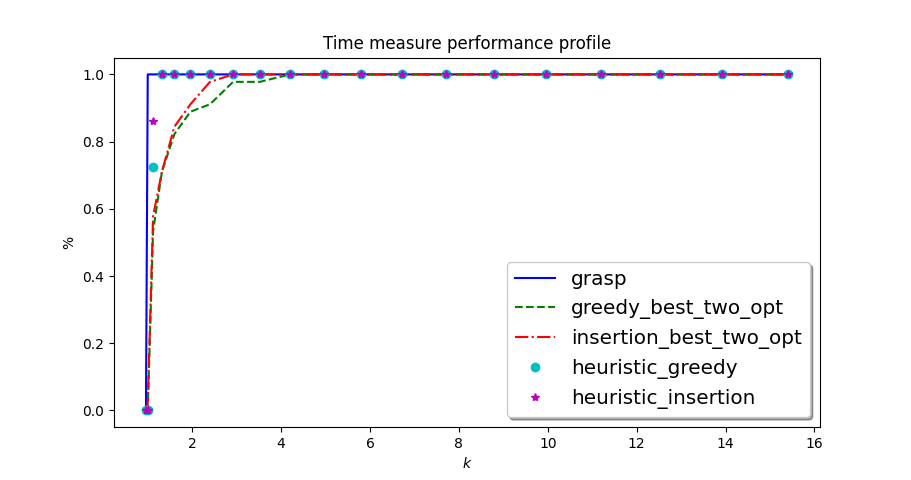
\includegraphics[width=\columnwidth]{../res/Lconstructives_refining_LA_time.png}
		\caption{Performance profile in time domain.}
		\label{fig:Lconstructives_refining_time}
	\end{subfigure}
	\begin{subfigure}{.7\textwidth}
		\centering
		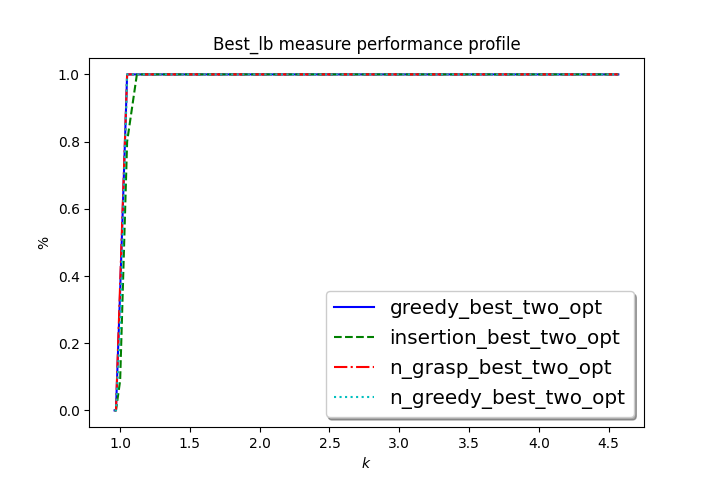
\includegraphics[width=\columnwidth]{../res/Lconstructives_refining_LA_lb.png}
		\caption{Performance profile in solution cost domain.}
		\label{fig:Lconstructives_refining_lb}
	\end{subfigure}
\caption{Performance profile of refining heuristic}
\label{fig:pp_Lconstructives_refining}
\end{figure}

The performance profile in fig. \ref{fig:pp_Lgreedy_refining} compare greedy algorithms with them \texttt{best\_two\_opt} optimization. It is clear that most of the execution time is required for the constructive heuristic, however the difference in term of cost optimization is done by the \texttt{best\_two\_opt}. In fig. \ref{fig:Lgreedy_refining_LA_lb} \texttt{n\_greedy\_best\_two\_opt} gain the solution of \texttt{greedy\_best\_two\_opt}, proving that it is not necessary to find the best tour created from the greedy, but is enough to compute ten random tour and than apply \texttt{best\_two\_opt} to find similar solution cost.

\begin{figure}
	\centering
	\begin{subfigure}{.8\textwidth}
		\centering
		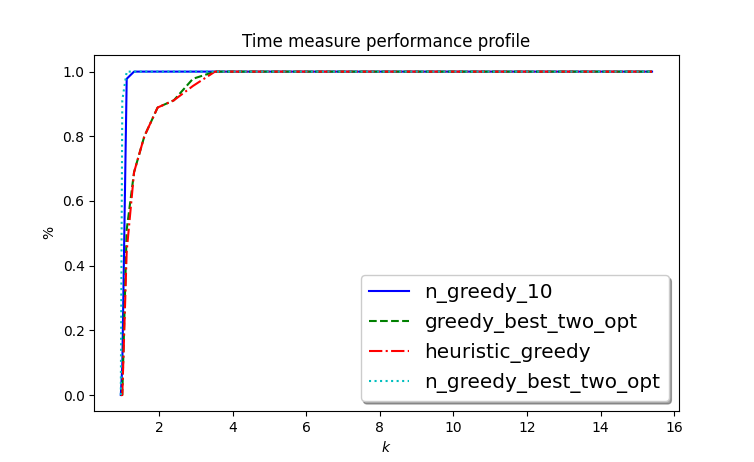
\includegraphics[width=\columnwidth]{../res/Lgreedy_refining_LA_time.png}
		\caption{Performance profile in solution cost domain.}
		\label{fig:Lgreedy_refining_LA_time}
	\end{subfigure}
	\begin{subfigure}{.8\textwidth}
		\centering
		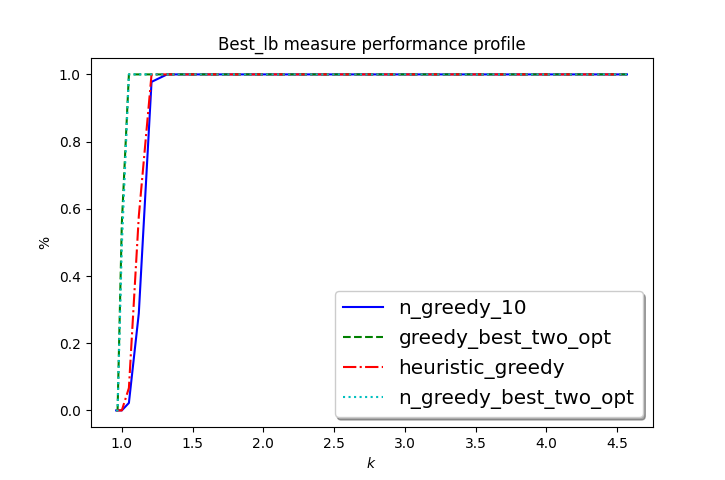
\includegraphics[width=\columnwidth]{../res/Lgreedy_refining_LA_lb.png}
		\caption{Performance profile in solution cost domain.}
		\label{fig:Lgreedy_refining_LA_lb}
	\end{subfigure}
	\caption{Comparison of constructive vs refining heuristics of greedy methods.}
	\label{fig:pp_Lgreedy_refining}
\end{figure}


The effectiveness of the refining heuristic depend from the warm start solution. In fig. \ref{fig:Lgrasp_insertion_refining_LA_lb} it is show that even if \texttt{heuristic\_insertion} generate shorter tour than \texttt{n\_grasp}, \texttt{n\_grasp\_best\_two\_opt} is better than \texttt{insertion\_best\_two\_opt}.

\begin{figure}
\centering
\begin{subfigure}{.7\textwidth}
	\centering
	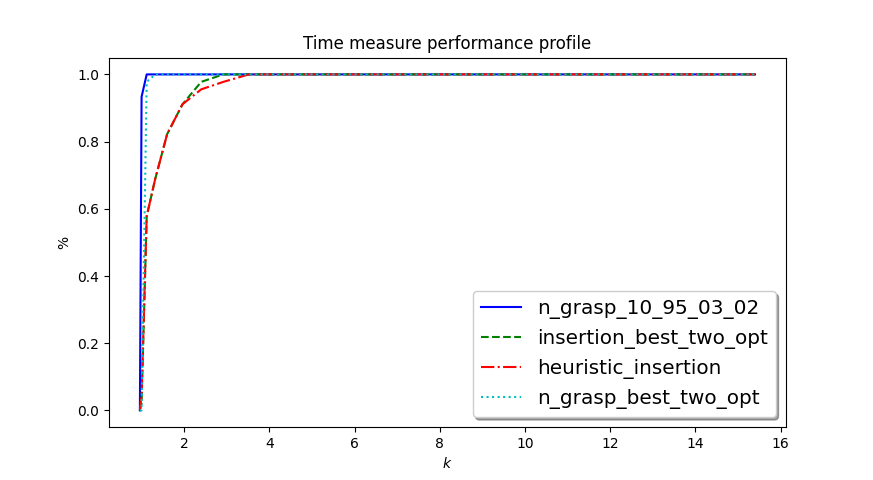
\includegraphics[width=\columnwidth]{../res/Lgrasp_insertion_refining_LA_time.png}
	\caption{Performance profile in solution cost domain.}
	\label{fig:Lgrasp_insertion_refining_LA_time}
\end{subfigure}
\begin{subfigure}{.7\textwidth}
	\centering
	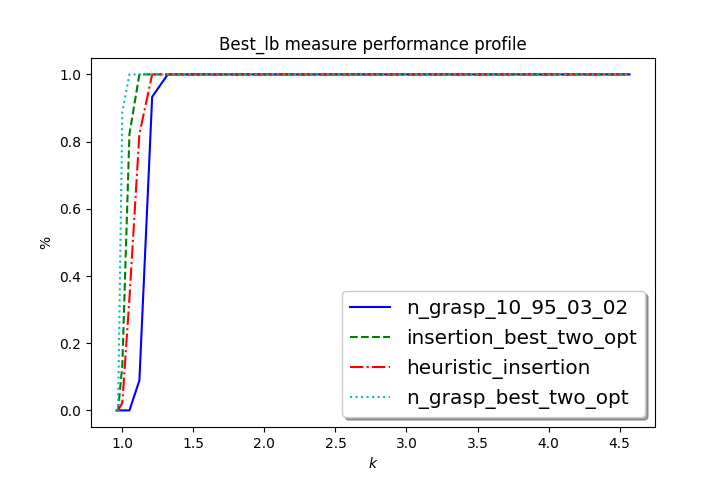
\includegraphics[width=\columnwidth]{../res/Lgrasp_insertion_refining_LA_lb.png}
	\caption{Performance profile in solution cost domain.}
	\label{fig:Lgrasp_insertion_refining_LA_lb}
\end{subfigure}
\caption{Comparison of constructive vs refining heuristics of grasp and insertion methods.}
\label{fig:pp_Lgrasp_insertion_refining}
\end{figure}

In conclusion, \texttt{best\_two\_opt} is a really useful refining heuristic for its time efficiency and cost effectiveness, however its effectiveness depend from how many cross edges has the warm start solution.
